\documentclass[10pt,oneside]{report}
\usepackage[left=3cm,top=0cm,right=3cm,nohead,nofoot]{geometry}
\geometry{a4paper}
%\geometry{landscape}
%\usepackage[parfill]{parskip}
\usepackage{graphicx}
\usepackage{subfigure}
\usepackage{wrapfig}
\usepackage[rflt]{floatflt}
\usepackage{enumerate}
\DeclareGraphicsExtensions{.png,.pdf,.jpg}
		
\usepackage{amssymb}

\usepackage[spanish]{babel}
\usepackage[utf8]{inputenc}
\usepackage[T1]{fontenc}


\usepackage{hyperref}

\begin{title} {\begin{center} \bf Escuela Superior Politecnica Del Litoral \linebreak \linebreak 
\includegraphics[width=.40\textwidth]{./imagenes/logo.jpg} \linebreak \linebreak \bf Reporte de Proyectos \linebreak \linebreak \bf Integrantes \end{center}}
\author{Danny Steven Ponce Marin \and Kevin Ricardo Silva Chavez \and Edwin Hermenejildo Reyes}
%\date{}
\end{title}

\begin{document}
\maketitle
\tableofcontents

\chapter{QT CREATOR - C++} JUEGO SUDOKU \newline
\textsf{SUDOKU \linebreak Sudoku es un pasatiempo que se publicó por primera vez a finales de la década de 1970 y se popularizó en Japón en 1986, dándose a conocer en el ámbito internacional en 2005 cuando numerosos periódicos empezaron a publicarlo en su sección de pasatiempos. Nosotros implementando Qt Creator para el diseño y C para la respectiva programacion logramos realizar nuestro propio diseño basándonos en todas las normal y reglas ya establecidas. La figura que se muestra a continuación es parte de nuestra interfaz gráfica.\linebreak \linebreak \begin{center}
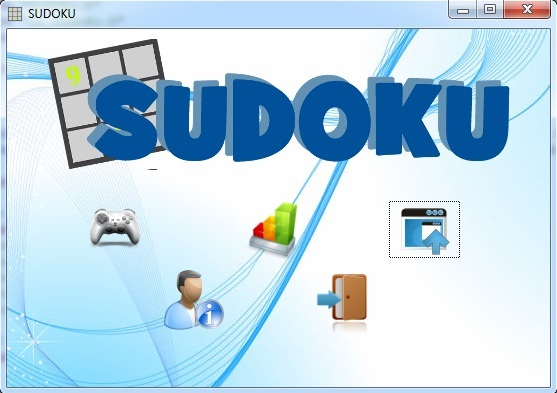
\includegraphics[width=.60\textwidth]{./imagenes/ventanaPrincipal.jpg}
\end{center}
\textsf { \linebreak El objetivo del sudoku es rellenar una cuadrícula de 9 * 9 (celdas 81 casillas) dividida en subcuadrículas de 3 x 3 (también llamadas "cajas" o "regiones") con las cifras del 1 al 9 partiendo de algunos números ya dispuestos en algunas de las celdas la figura que se muestra a continuación nos ayudará a entender mejor lo explicado anteriormente. \newline \begin{center}
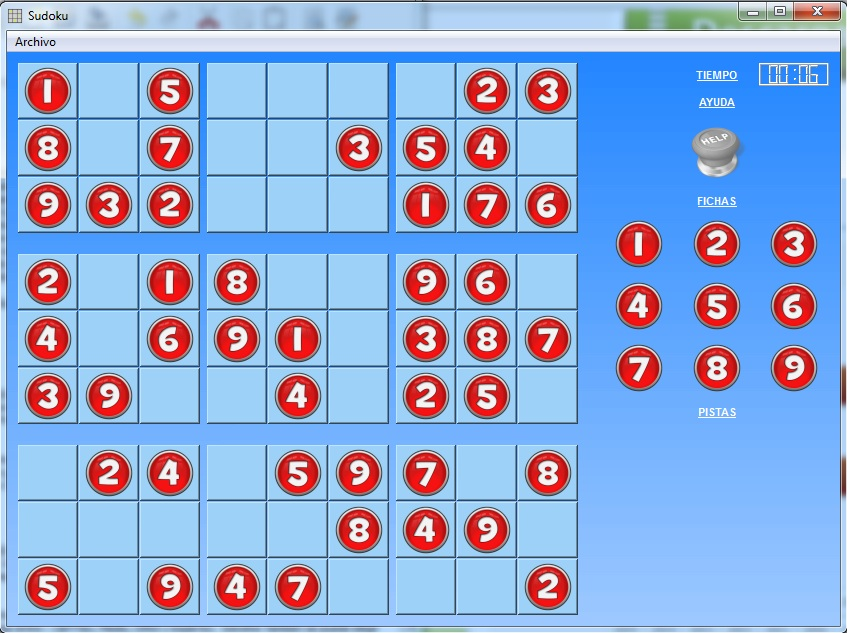
\includegraphics[width=.60\textwidth]{./imagenes/facil.jpg}
\end{center}}
\begin{figure}
\textsf{\linebreak Aunque se podrían usar colores, letras, figuras, se conviene en usar números para mayor claridad, lo que importa, es que sean nueve elementos diferenciados, que no se deben repetir en una misma fila, columna o subcuadrícula. Un sudoku está bien planteado si la solución es única. La solución de un sudoku siempre es un cuadrado latino, aunque el recíproco en general no es cierto ya que el sudoku establece la restricción añadida de que no se puede repetir un mismo número en una región. Vease la figura 1.1. \newline
\begin{center}
\subfigure[Alerta Inválida: Fila]{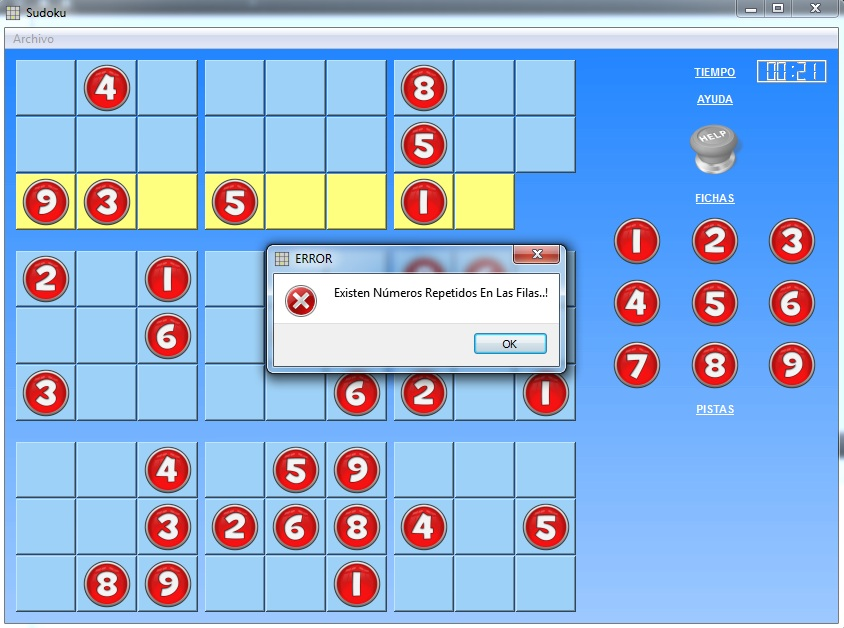
\includegraphics[width=50mm]{./imagenes/alertaFila.jpg}}
\subfigure[Alerta Inválida: Columna]{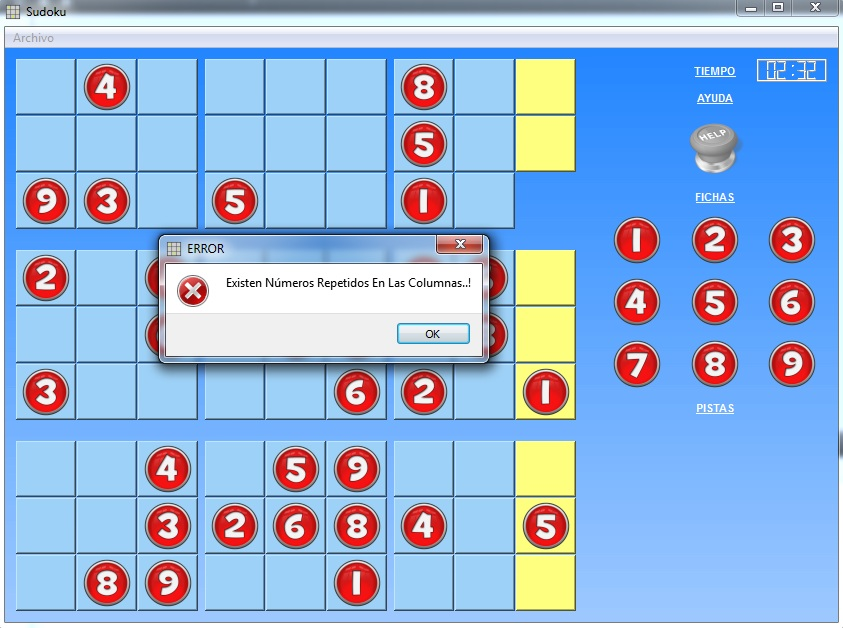
\includegraphics[width=50mm]{./imagenes/alertaColumna.jpg}}
\subfigure[Alerta Inválida: Sub-Cuadricula]{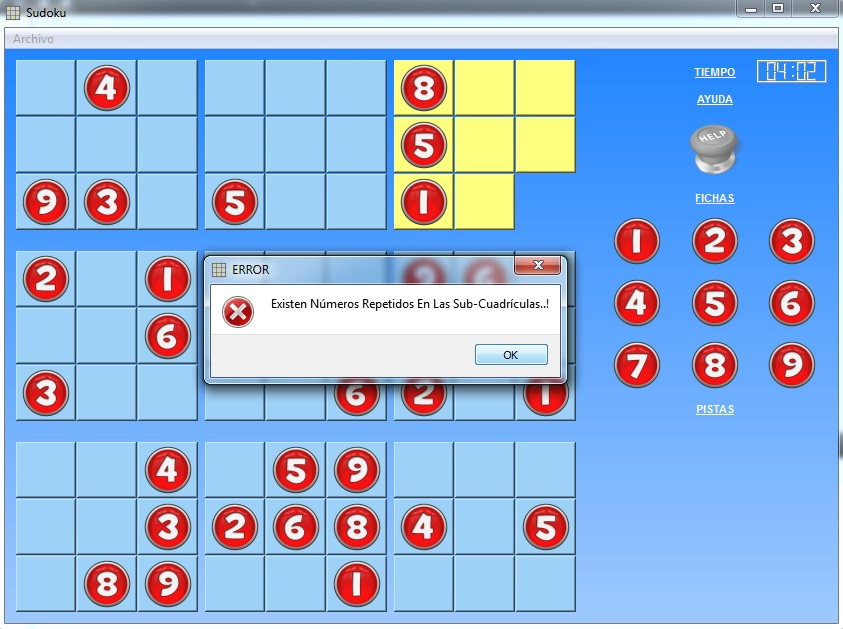
\includegraphics[width=50mm]{./imagenes/alertaSubcuadricula.jpg}}
\subfigure[Alerta Incorrecta]{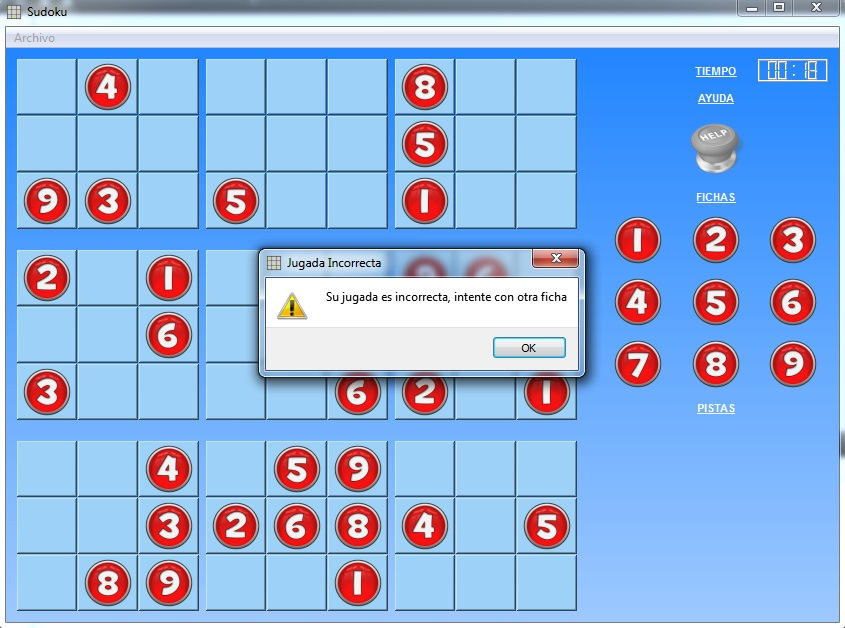
\includegraphics[width=50mm]{./imagenes/alertaIncorrecta.jpg}}
\caption{Tipos de Alerta.}
\end{center}}
\end{figure}
\begin{bf} Niveles de Dicicultad .\end{bf}\newline Los programas informáticos que resuelven sudokus pueden estimar la dificultad que tiene un humano para encontrar la solución, basándose en la complejidad de las técnicas de resolución necesarias. Esta estimación permite a los editores adaptar sus sudokus para personas con diferente experiencia resolutoria. Algunas versiones en línea también ofrecen varios niveles de dificultad. \newline \begin{center} 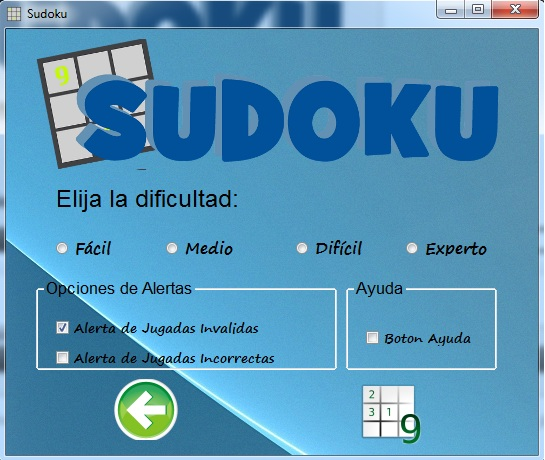
\includegraphics[width=.60\textwidth]{./imagenes/nuevoJuego.jpg} \end{center} \begin{figure}[h] \begin{center} \subfigure[Fácil]{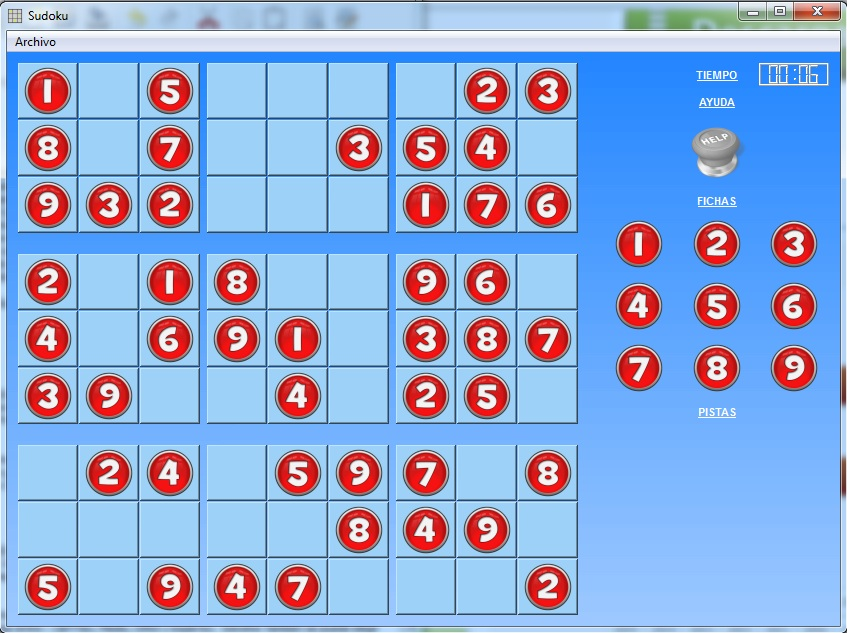
\includegraphics[width=50mm]{./imagenes/facil.jpg}}
\subfigure[ Medio]{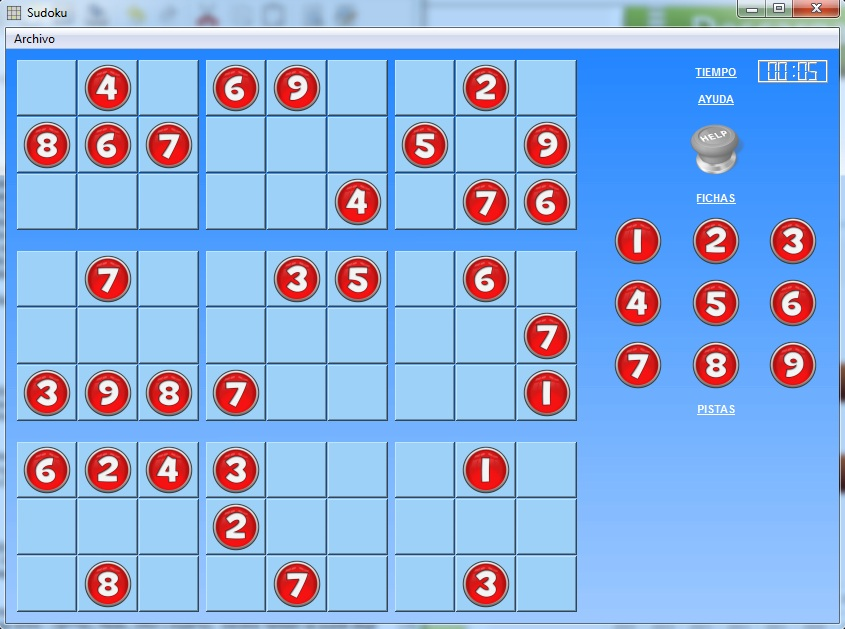
\includegraphics[width=50mm]{./imagenes/medio.jpg}}
\subfigure[Difícil]{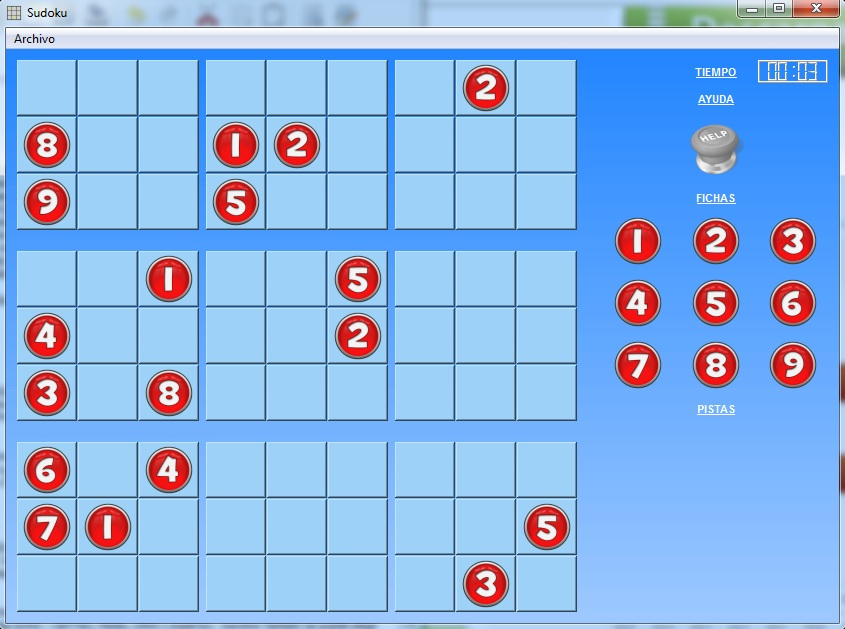
\includegraphics[width=50mm]{./imagenes/dificil.jpg}}
\subfigure[Experto]{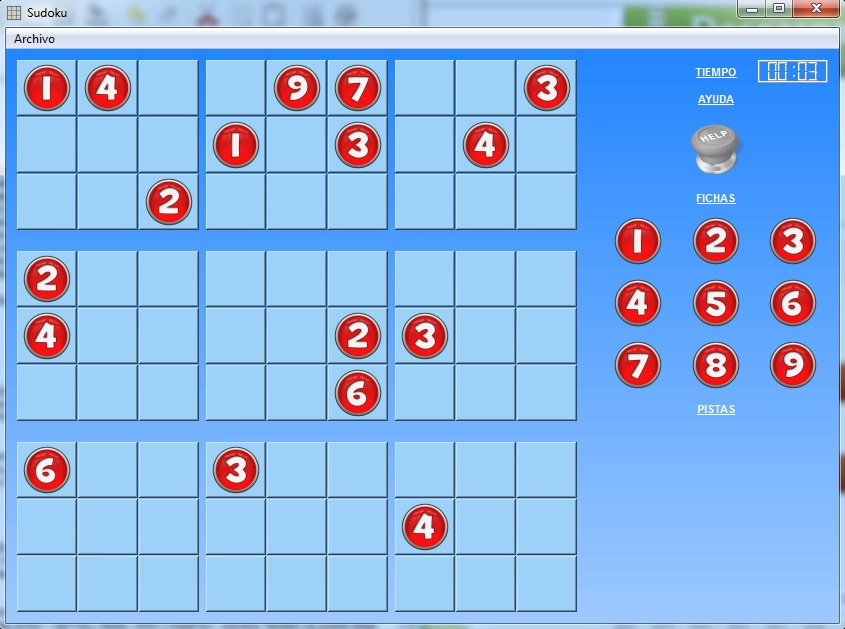
\includegraphics[width=50mm]{./imagenes/experto.jpg}}
\caption{Niveles de Dificultad.} \end{center}\end{figure} \newpage \begin{bf} Relación de Equivalencia Entre los Sudokus.\end{bf}\newline \newline Decimos que dos Sudokus son equivalentes si uno de ellos puede ser transformado en otro por medio de composiciones de las siguientes transformaciones:\newline Permutación de los dígitos 1; 2;……; 9.\newline Reflexión.\linebreak Rotación (0, 90, 180 y 270).\newline Permutación de las columnas 1 a 3, 4 a 6 ó 7 a 9.\newline Permutación de las filas 1 a 3, 4 a 6 ó 7 a 9.\newline \newline}

\chapter{PYTHON}JUEGO SUDOKU \newline
\textsf{SUDOKU \linebreak Sudoku es un pasatiempo que se publicó por primera vez a finales de la década de 1970 y se popularizó en Japón en 1986, dándose a conocer en el ámbito internacional en 2005 cuando numerosos periódicos empezaron a publicarlo en su sección de pasatiempos. Nosotros implementando Qt Creator para el diseño y C para la respectiva programacion logramos realizar nuestro propio diseño basándonos en todas las normal y reglas ya establecidas. La figura que se muestra a continuación es parte de nuestra interfaz gráfica.\linebreak \linebreak \begin{center}
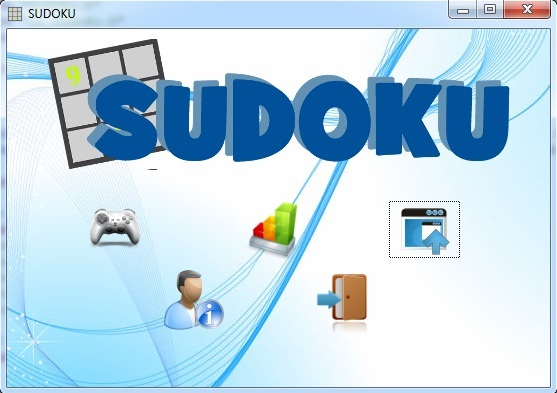
\includegraphics[width=.60\textwidth]{./imagenes/ventanaPrincipal.jpg}
\end{center}
\textsf { \linebreak El objetivo del sudoku es rellenar una cuadrícula de 9 * 9 (celdas 81 casillas) dividida en subcuadrículas de 3 x 3 (también llamadas "cajas" o "regiones") con las cifras del 1 al 9 partiendo de algunos números ya dispuestos en algunas de las celdas la figura que se muestra a continuación nos ayudará a entender mejor lo explicado anteriormente. \newline \begin{center}
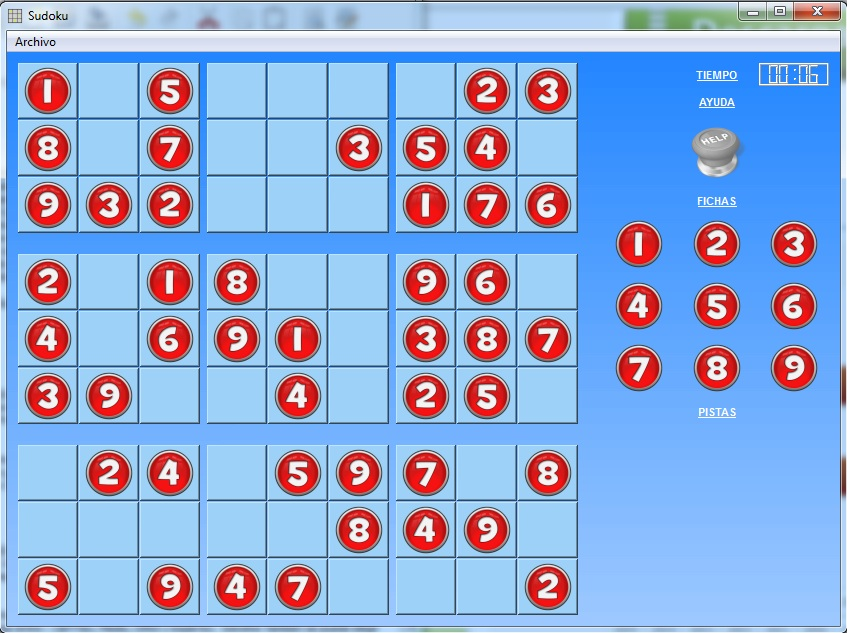
\includegraphics[width=.60\textwidth]{./imagenes/facil.jpg}
\end{center}}
\begin{figure}
\textsf{\linebreak Aunque se podrían usar colores, letras, figuras, se conviene en usar números para mayor claridad, lo que importa, es que sean nueve elementos diferenciados, que no se deben repetir en una misma fila, columna o subcuadrícula. Un sudoku está bien planteado si la solución es única. La solución de un sudoku siempre es un cuadrado latino, aunque el recíproco en general no es cierto ya que el sudoku establece la restricción añadida de que no se puede repetir un mismo número en una región. Vease la figura 1.1. \newline
\begin{center}
\subfigure[Alerta Inválida: Fila]{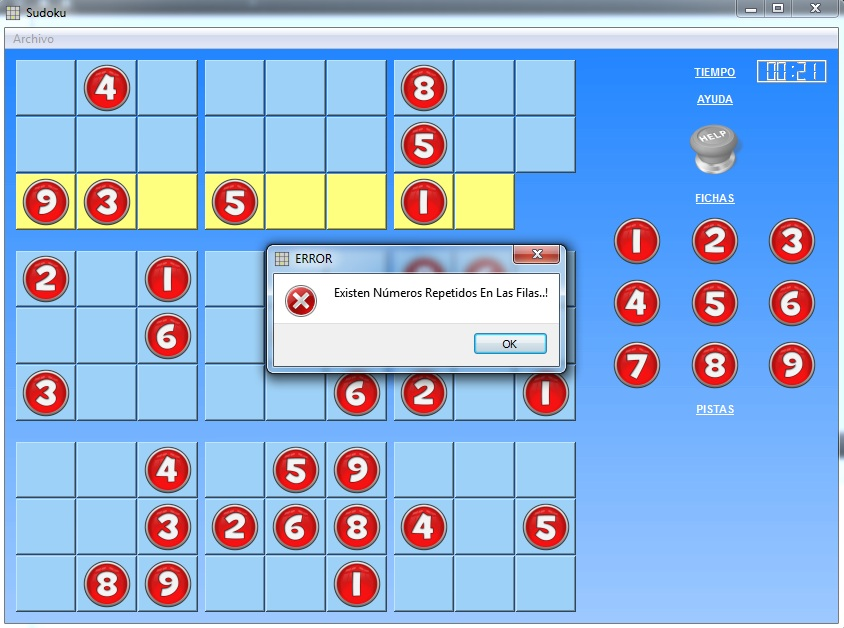
\includegraphics[width=50mm]{./imagenes/alertaFila.jpg}}
\subfigure[Alerta Inválida: Columna]{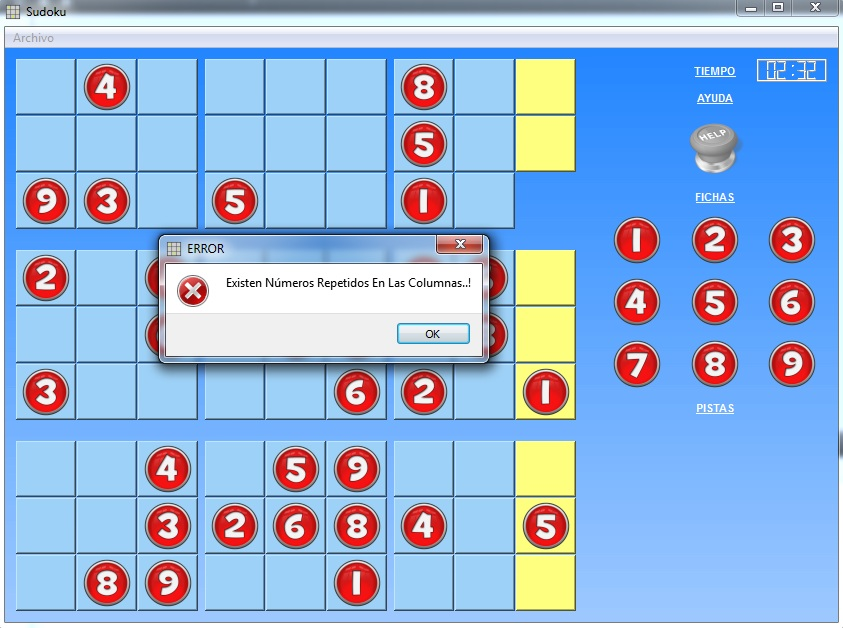
\includegraphics[width=50mm]{./imagenes/alertaColumna.jpg}}
\subfigure[Alerta Inválida: Sub-Cuadricula]{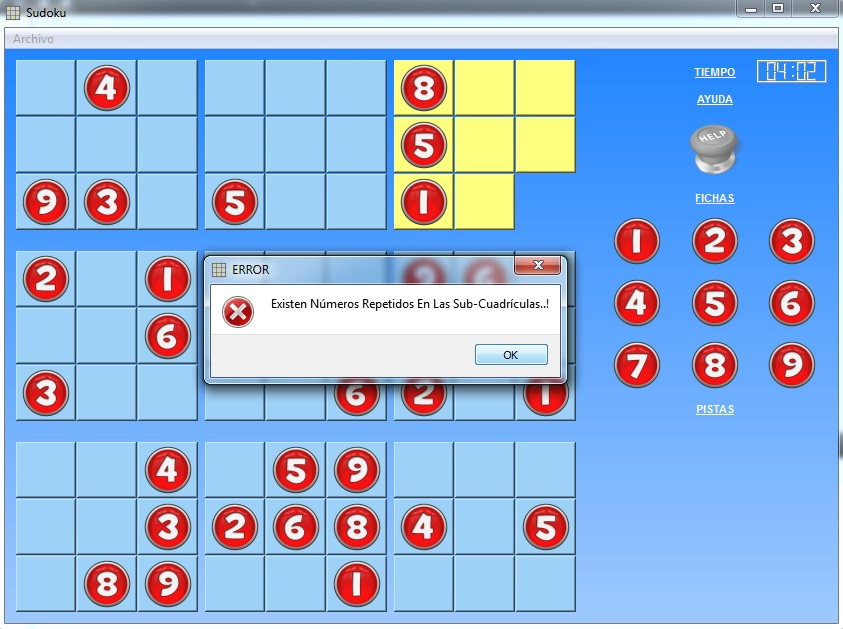
\includegraphics[width=50mm]{./imagenes/alertaSubcuadricula.jpg}}
\subfigure[Alerta Incorrecta]{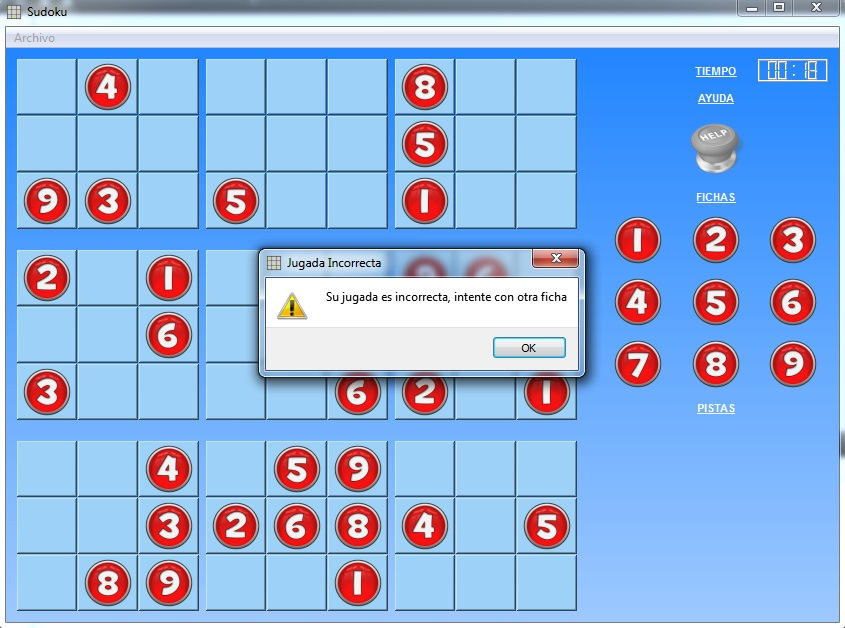
\includegraphics[width=50mm]{./imagenes/alertaIncorrecta.jpg}}
\caption{Tipos de Alerta.}
\end{center}}
\end{figure}
\begin{bf} Niveles de Dicicultad .\end{bf}\newline Los programas informáticos que resuelven sudokus pueden estimar la dificultad que tiene un humano para encontrar la solución, basándose en la complejidad de las técnicas de resolución necesarias. Esta estimación permite a los editores adaptar sus sudokus para personas con diferente experiencia resolutoria. Algunas versiones en línea también ofrecen varios niveles de dificultad. \newline \begin{center} 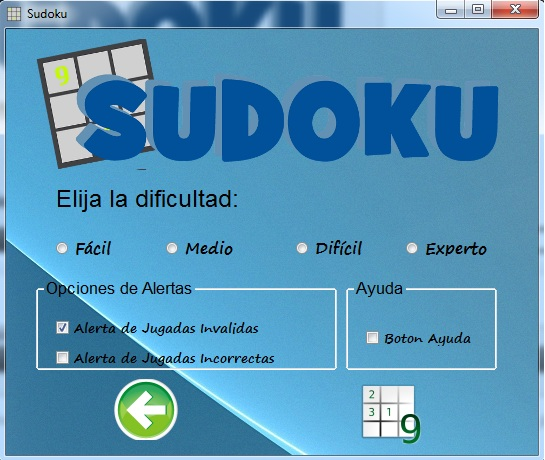
\includegraphics[width=.60\textwidth]{./imagenes/nuevoJuego.jpg} \end{center} \begin{figure}[h] \begin{center} \subfigure[Fácil]{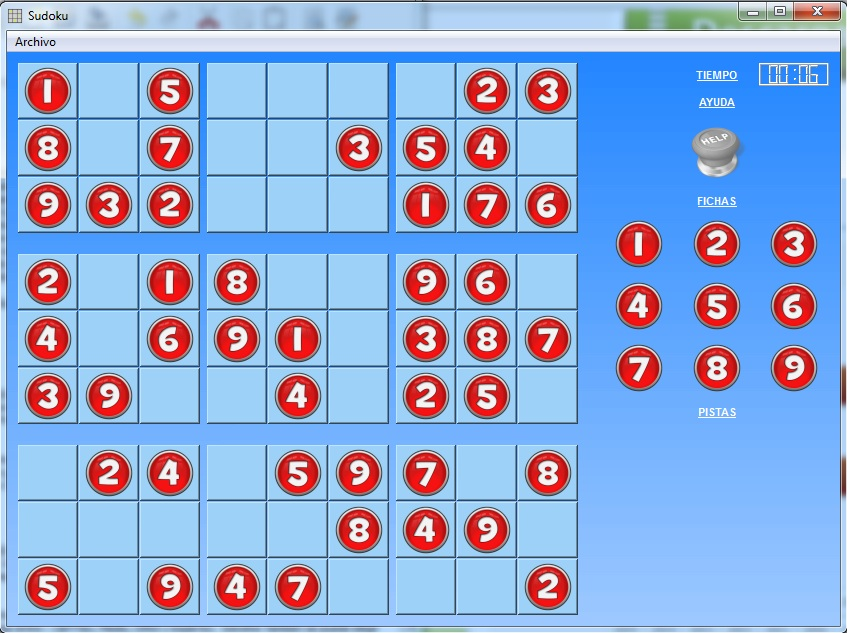
\includegraphics[width=50mm]{./imagenes/facil.jpg}}
\subfigure[ Medio]{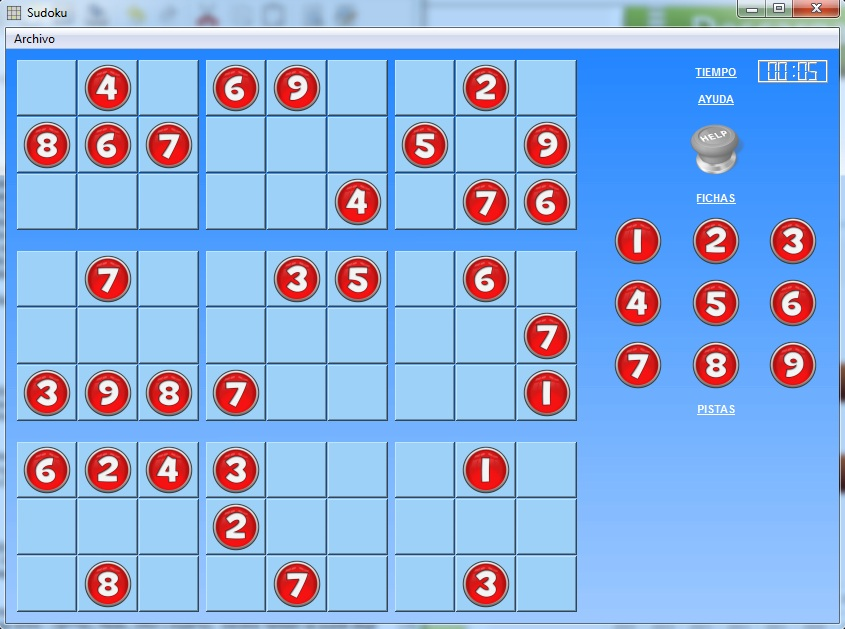
\includegraphics[width=50mm]{./imagenes/medio.jpg}}
\subfigure[Difícil]{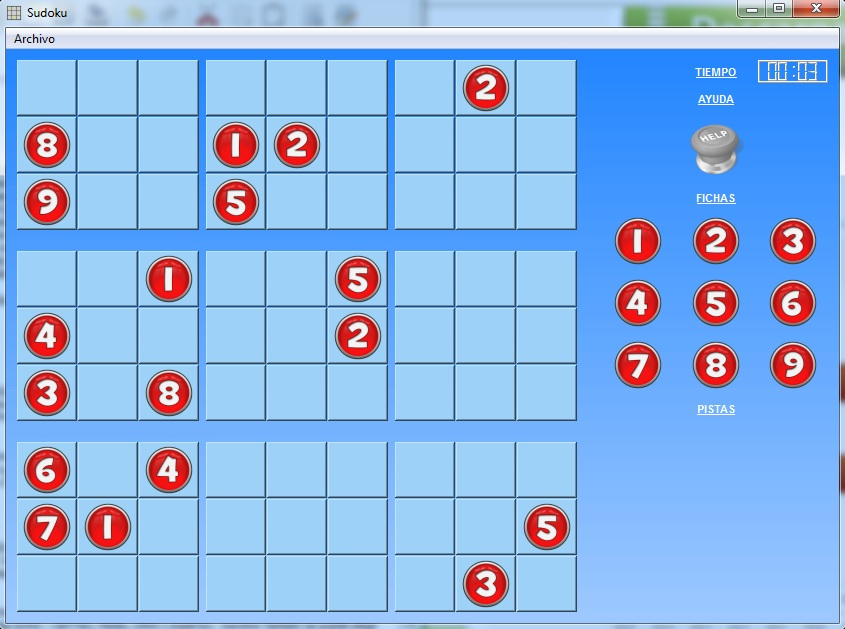
\includegraphics[width=50mm]{./imagenes/dificil.jpg}}
\subfigure[Experto]{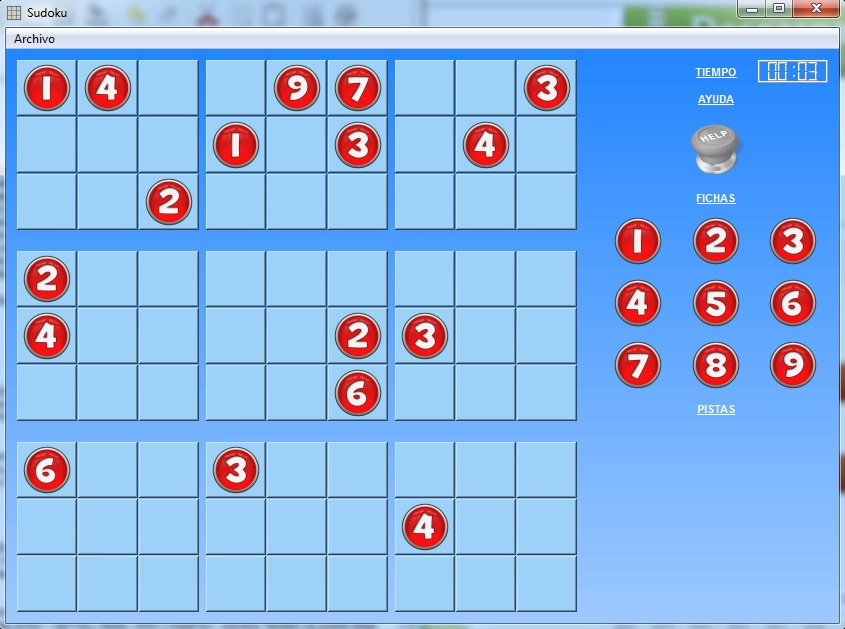
\includegraphics[width=50mm]{./imagenes/experto.jpg}}
\caption{Niveles de Dificultad.} \end{center}\end{figure} \newpage \begin{bf} Relación de Equivalencia Entre los Sudokus.\end{bf}\newline \newline Decimos que dos Sudokus son equivalentes si uno de ellos puede ser transformado en otro por medio de composiciones de las siguientes transformaciones:\newline Permutación de los dígitos 1; 2;……; 9.\newline Reflexión.\linebreak Rotación (0, 90, 180 y 270).\newline Permutación de las columnas 1 a 3, 4 a 6 ó 7 a 9.\newline Permutación de las filas 1 a 3, 4 a 6 ó 7 a 9.\newline \newline}

\chapter{HASKELL:  Analizador Léxico}
\textsf{Haskell es un lenguaje de programación estandarizado multi-propósito puramente funcional con semánticas no estrictas y fuerte tipificación estática. Su nombre se debe al lógico estadounidense Haskell Curry. En Haskell, "una función es un ciudadano de primera clase" del lenguaje de programación. Como lenguaje de programación funcional, el constructor de controles primario es la función. Las características más interesantes de Haskell incluyen el soporte para tipos de datos y funciones recursivas, listas, tuplas, guardas y calce de patrones. La combinación de las mismas pueden resultar en algunas funciones casi triviales cuya versión en lenguajes imperativos pueden llegar a resultar extremadamente tediosas de programar. Haskell es, desde 2002, uno de los lenguajes funcionales sobre los que más se ha investigado. \newline  \newline
\begin{bf}  Analizador Léxico. \end{bf} \newline \newline Un analizador léxico es el encargado de leer carácter por carácter de un archivo fuente (escrito en C) y construir elementos léxicos llamados \begin{bf} Patrones \end{bf} que serán utilizados posteriormente por un analizador sintáctico.\newline
Un \begin{bf} patrón \end{bf} es una pareja ordenada compuesta por un token y un lexema.\newline
Un \begin{bf} token \end{bf} es el elemento léxico del lenguaje, es decir el símbolo terminal de una gramática libre de contexto (GLC).\newline
Y un \begin{bf} lexema \end{bf} es la secuencia de caracteres que coinciden con un token. \newline \newline
 \begin{bf} Gramática Léxica \end{bf} \newline \newline
La especificación de un lenguaje de programación a menudo incluye un conjunto de reglas que definen el léxico. Estas reglas consisten comumente enexpresiones regulares que indican el conjunto de posibles secuencias de caracteres que definen un token o lexema. En algunos lenguajes de programación es necesario establecer patrones para caracteres especiales (como el espacio en blanco) que la gramática pueda reconocer sin que constituya un token en sí. \newline \newline
\begin{bf} Análisis \end{bf} \newline \newline
Esta etapa está basada usualmente en una máquina de estados finitos. Esta máquina contiene la información de las posibles secuencias de caracteres que puede conformar cualquier token que sea parte del lenguaje (las instancias individuales de estas secuencias de caracteres son denominados lexemas). Por ejemplo, un token de naturaleza entero puede contener cualquier secuencia de caracteres numéricos.
\begin{figure}[t]
	\centering
	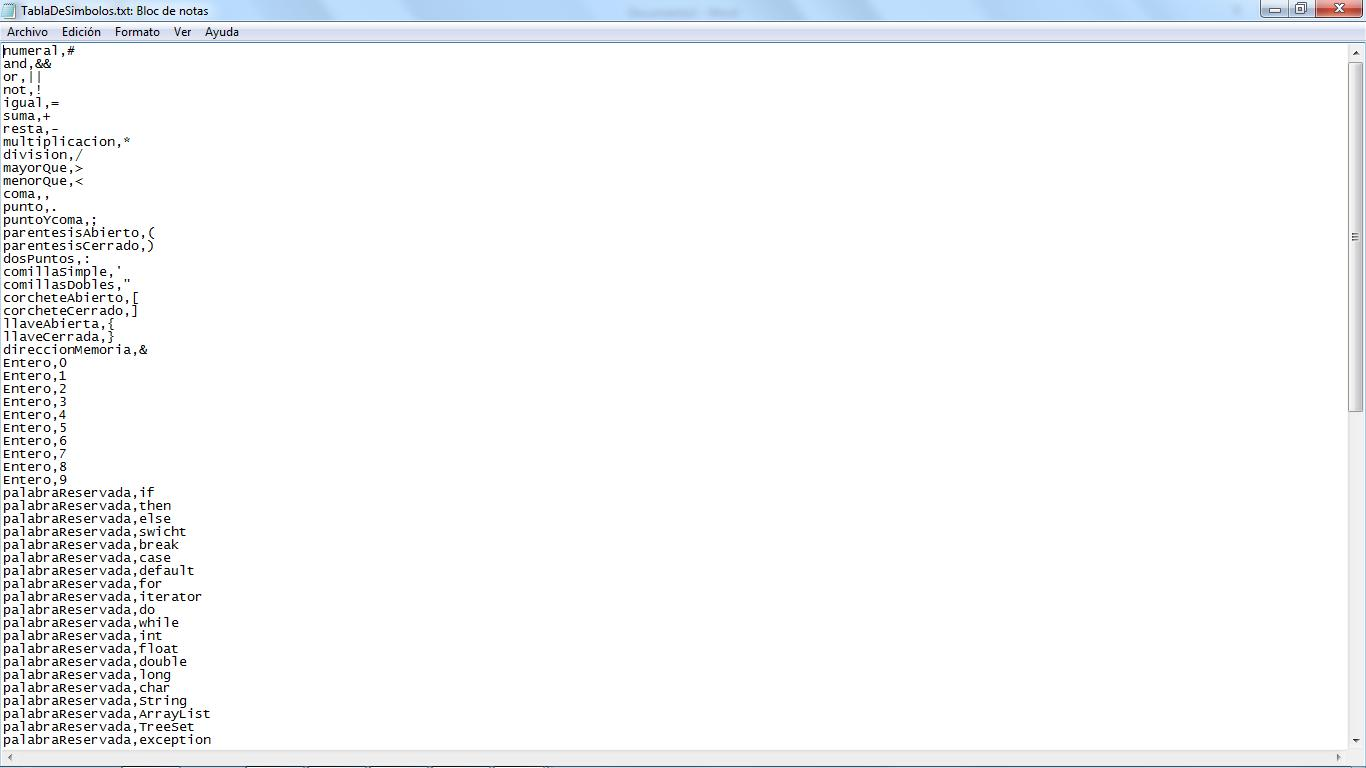
\includegraphics[width=.80\textwidth]{./imagenes/haskell1.jpg}
	\caption{Tabla de Símbolos}
	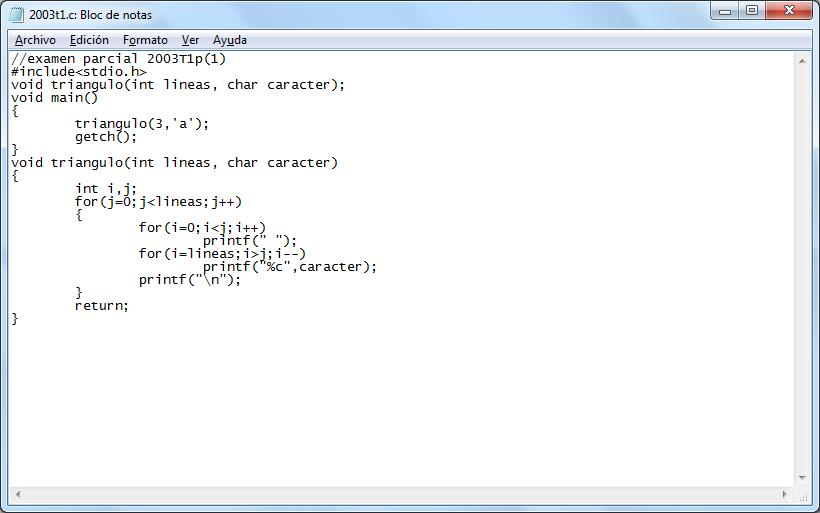
\includegraphics[width=.80\textwidth]{./imagenes/haskell2.jpg}
	\caption{Archivo}
	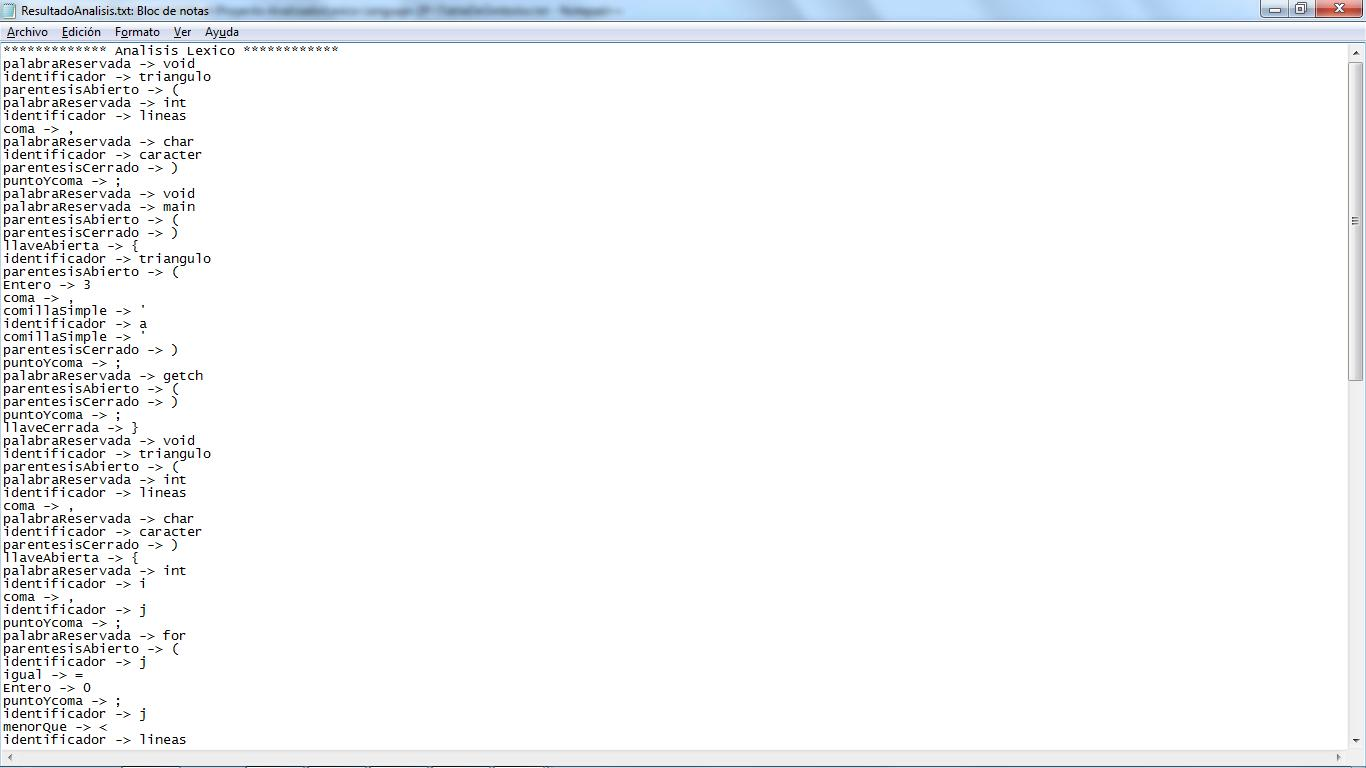
\includegraphics[width=.80\textwidth]{./imagenes/haskell3.jpg}
	\caption{Resultado de Analisis}
\end{figure}
}

\chapter{LATEX} DOCUMENTACIÓN \newline
\textsf{\footnote{\url{http://http://es.wikipedia.org/wiki/LaTeX}} Es un sistema de composición de textos, orientado especialmente a la creación de libros, documentos científicos y técnicos que contengan fórmulas matemáticas. \begin{center} 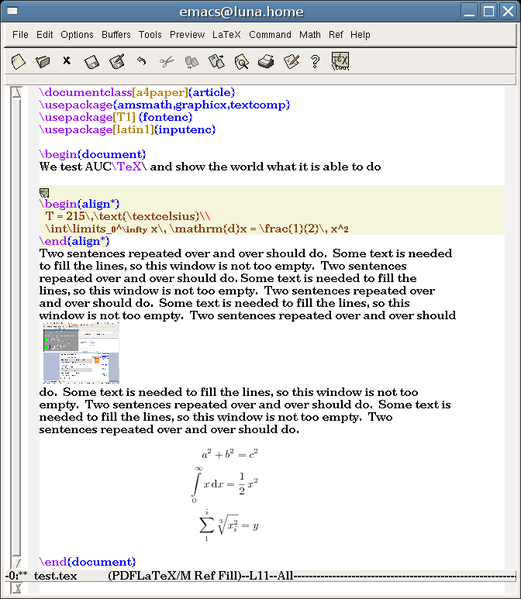
\includegraphics[width=.60\textwidth]{./imagenes/latex.jpg} \newline \end{center} \begin{bf} Descripción. \end{bf} \newline \newline LaTeX es un sistema de composición de textos que está formado mayoritariamente por órdenes construidas a partir de comandos de TeX - un lenguaje «de nivel bajo», en el sentido de que sus acciones últimas son muy elementales— pero con la ventaja añadida de «poder aumentar las capacidades de LaTeX utilizando comandos propios del TeX descritos en The TeXbook». Esto es lo que convierte a LaTeX en una herramienta práctica y útil pues, a su facilidad de uso, se une toda la potencia de TeX. Estas características hicieron que LaTeX se extendiese rápidamente entre un amplio sector científico y técnico, hasta el punto de convertirse en uso obligado en comunicaciones y congresos, y requerido por determinadas revistas a la hora de entregar artículos académicos.
Su código abierto permitió que muchos usuarios realizasen nuevas utilidades que extendiesen sus capacidades con objetivos muy variados, a veces ajenos a la intención con la que fue creado: aparecieron diferentes dialectos de LaTeX que, a veces, eran incompatibles entre sí.\newpage
\begin{bf} Uso. \end{bf} \newline \newline
\begin{floatingfigure}[r]{4.5cm}
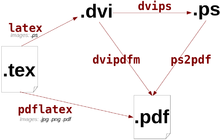
\includegraphics{./imagenes/formato.jpg}
\caption{Tipo de Formatos}
\end{floatingfigure}
El modo en que LaTeX interpreta la «forma» que debe tener el documento es medianteetiquetas. Por ejemplo, documentclass{article} le dice a LaTeX que el documento que va a procesar es un artículo. Puede resultar extraño que hoy en día se siga usando algo que no es WYSIWYG, pero las características de LaTeX siguen siendo muchas y muy variadas. También hay varias herramientas (aplicaciones) que ayudan a una persona a escribir estos documentos de una manera más visual (LyX, TeXmacs y otros). A estas herramientas se les llama WYSIWYM(«lo que ves es lo que quieres decir»).
Una de las ventajas de LaTeX es que la salida que ofrece es siempre la misma, con independencia del dispositivo (impresora, pantalla, etc.) o el sistema operativo (MS Windows,MacOS, Unix, GNU/Linux, etc.) y puede ser exportado a partir de una misma fuente a numerosos formatos tales como Postscript, PDF, SGML, HTML, RTF, etc. Existen distribuciones e IDEs de LaTeX para todos los sistemas operativos más extendidos, que incluyen todo lo necesario para trabajar. Hay, por ejemplo, programas para Windows como TeXnicCenter, para Linux como Kile, o para MacOS como TeXShop, todos liberados bajo la Licencia GPL. Existe además un editor multiplataforma (para MacOS, Windows y Unix) llamado Texmaker, que también tiene licencia GPL. \newline \newline
\begin{bf} Lenguaje. \end{bf} \newline \newline La forma más práctica de escribir tildes y otros símbolos que no aparecen en el alfabeto inglés, es obviamente escribiéndolos directamente del teclado.
\begin{figure}[h]
	\centering
	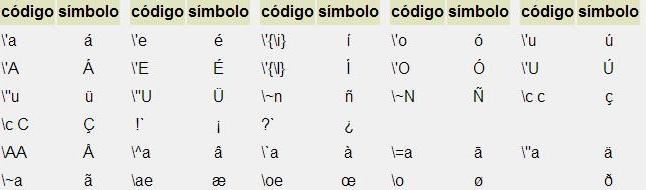
\includegraphics[width=.80\textwidth]{./imagenes/lenguaje1.jpg}
	\caption{Lenguaje}
	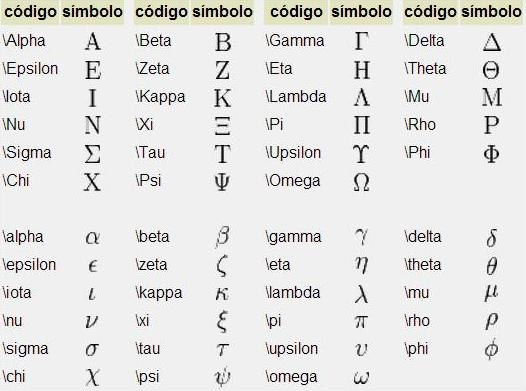
\includegraphics[width=.60\textwidth]{./imagenes/lenguaje2.jpg}
	\caption{Alfabeto griego}
\end{figure}
\begin{figure}[t]
	\centering
	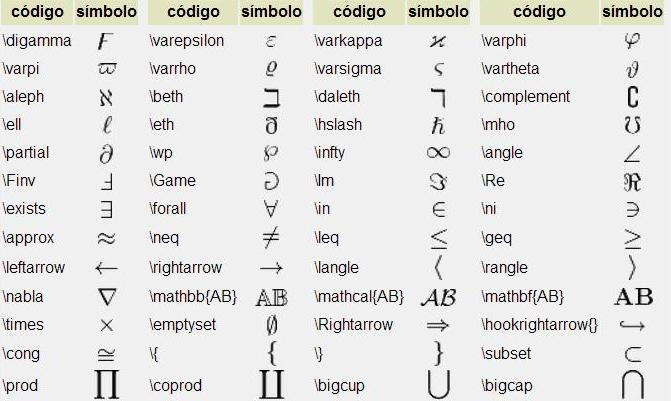
\includegraphics[width=.80\textwidth]{./imagenes/lenguaje3.jpg}
	\caption{Símbolos matemáticos}
	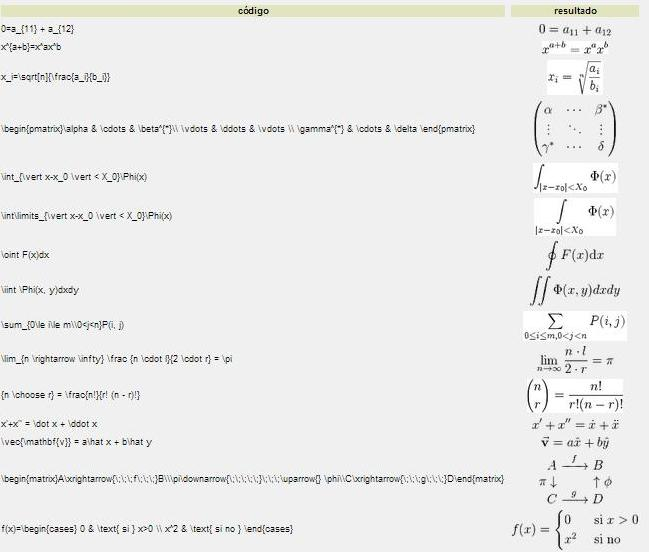
\includegraphics[width=.80\textwidth]{./imagenes/lenguaje4.jpg}
	\caption{Expresiones matemáticas}
\end{figure}
}


\chapter{Experiencias}
{\bf Danny Steven Ponce Marin \newline }
\begin{itemize}\renewcommand{\labelitemi}{$\bullet$}
	\item {\bf Github.-} \textsf{ Github es un gran lugar para trabajar con los proyectos y nos permite integrar colaboradores que ayuden al desarrollo de un proyecto. Todo proyecto que desarrollamos en esta materia lo manejamos mediante un repositorio y cada integrante hacia una nueva versión del proyecto y los demás integrantes obteníamos la última actualización del proyecto y así sucesivamente trabajamos en grupo. Como experiencia de trabajar con Github con la herramienta de escritorio para Windows se me hizo muy fácil, interesante y útil ya que nos ayuda a que el grupo pueda trabajar específicamente en una parte del proyecto y no solo en una maquina trabajar. Hacer commits en Github es  de gran utilidad ya que cada integrante se da cuenta del cambio que realizo al proyecto e incluso las líneas de código que cambiaron o la inserción de un nuevo archivo. Además de eso podemos ver las aportaciones de cada integrante del grupo mediante sus commits que ha trabajado por medio de un gráfico y muchas cosas más interesantes. Mi conclusión de utilizar Github para nuestros proyectos es de gran ayuda en especial al trabajar en grupo.}
	\item {\bf Latex.-}\textsf{ Un lenguaje de programación de bajo nivel con un sistema de composición de textos orientado especialmente a la creación de libros, documentos, etc. Al inicio algo complicado debido a la costumbre de trabajar en Word o Power Point pero con práctica se tornó interesante debido los resultados que toma en su presentación. Una herramienta muy práctica y utilizada a nivel profesional. Utiliza comandos propios, posee capacidades gráficas para representar ecuaciones y formulas complicadas pero con la dificultad para colocar en el documento caracteres especiales como tildes, etc. Lo cual hay que hacerlos con comandos especiales.}
	\item {\bf QT.-}\textsf{  Es un IDE multiplataforma que se ajusta a las necesidades de los desarrolladores. Un lenguaje consciente de la estructura de muchas clases de Qt, lo que aumenta la capacidad de mostrar los datos con claridad, permite diseñar rápidamente widgets y diálogos usando los mismos widgets que se usó en la aplicación. Los formularios son totalmente funcionales y pueden ser previsualizados inmediatamente para asegurarse de que se verá y sentirá exactamente como usted lo pensó  }
	\item {\bf Python.-}  \textsf{ Me resulto fácil programar en este lenguaje debido a que ya lo había visto,  tiene muchas ventajas, el que no es declarativo. La manera de trabajar con las tabulaciones debido a que no existe un delimitador que me diga que ya termino una estructura. La instalación PyQt, no fue fácil y me dio muchos problemas las versiones de python, PyDev y eclipse, que fue el IDE en donde se desarrolló. El paso de código desde C++ a Python fue tedioso ya que se tenía que investigar ciertas formas de implementar que las hacíamos en C++ (lenguaje orientado a objetos) y no las podíamos hacer en Python.}
	\item {\bf Haskell.-}\textsf{ Haskell lo defino un lenguaje moderno, interesante y sobre todo recursivo. Se me hizo difícil de comprender al inicio porque estaba acostumbrado al uso de ciclos. Las complicaciones que tuve durante el proyecto fue sacar condiciones bases y la recursiva. Después de entender bien su sintaxis y la forma de ver las cosas recursivamente se me hizo muy fácil el desarrollo del proyecto. El manejo de listas dentro de Haskell es muy útil a través de la cabeza y cola de dicha lista. Este lenguaje me ayudó mucho a entender la recursividad para resolver un problema. } 
\end{itemize}\newpage
{\bf Edwin Hermenejildo Reyes \newline }
\begin{itemize}\renewcommand{\labelitemi}{$\bullet$}
	\item {\bf Github.-}\textsf{Es un sistema de control de versiones distribuido cuyo objetivo es el de permitir mantener una gran cantidad de código a una gran cantidad de programadores eficientemente. Un hosting online para nuestros repositorios que utiliza Git para el mantenimiento y versionado del código fuente, añadiendo una serie de servicios extras para la gestión del proyecto y el código fuente. La principal ventaja es tener centralizado el desarrollo de forma que todo el equipo pueda enviar y comprobar cambios de forma sencilla sin necesidad de ver uno a uno los cambios en los equipos de cada desarrollador.}
	\item {\bf Latex.-}\textsf{Un lenguaje de bajo nivel muy interesante debido a su sistema de composición de textos orientado especialmente a la creación de documentos, libros, reportes, etc. Al inicio muy tedioso debido a la costumbre de trabajar en Word o Power Point pero con práctica se tornó interesante debido a la forma y  estructura que toma en su presentación. Una herramienta muy práctica y utilizada a nivel profesional según mi investigación. Utiliza comandos propios, posee capacidades gráficas para representar ecuaciones y formulas complicadas pero su interfaz gráfica es muy pobre.}
	\item {\bf QT.-}\textsf{Me resulto fácil debido a una experiencia de trabajo casi similar con programación orientada a objetos. Con una buena investigación de como enlazar QT con C++ se torna interesante el trabajo. Tuve inconvenientes al momento de conectar la parte de la vista que las hacíamos con el QtDesigner con el modelo ya que utilizamos el modelo MVC para la creación de nuestro proyecto, utilizar los connects, las signals y los slots fue para mí lo más complicado con respecto al aprendizaje de este lenguaje. }
	\item {\bf Python.-}\textsf{Me resulto difícil  programar en este lenguaje debido a que no lo había visto,  tiene muchas ventajas debido a que la declaración de variables no es necesaria. Un programa muy ordenado debido a su identación por lo que no existe un delimitador que me diga que ya termino una estructura. La instalación PyQt, no fue fácil y me dio muchos problemas las versiones de python, PyDev y eclipse, que fue el IDE en donde se desarrolló. El paso de código desde C++ a Python fue tedioso ya que se tenía que investigar ciertas formas de implementar que las hacíamos en C++ (lenguaje orientado a objetos) y no las podíamos hacer en Python.}
	\item {\bf Haskell.-}\textsf{Es un lenguaje funcional de aprendizaje muy difícil. Tenía un cruce de ideas muy contradictorias debido a los lenguajes que había estudiado. Haskell, por el hecho de que es funcional, todo es en base a funciones, no se pueden usar bucles ni estructuras de repetición, todo es en base a la recursividad. Su sintaxis muy dificil de aprender ya que es diferente a como programaba. una ventaja de éste lenguaje es que como todo es recursivo, las funciones resultan realmente pequeñas en comparación con otros lenguajes.} 
\end{itemize}\newpage
{\bf Kevin Ricardo Silva Chavez \newline }
\begin{itemize}\renewcommand{\labelitemi}{$\bullet$}
	\item {\bf Github.-} \textsf{Este sistema de versionamiento que me tocó utilizar en este parcial, cabe recalcar que no fue nuevo para mí ya que en el semestre pasado también lo vi, y en este semestre fue el sistema de versionamiento escogido para otra materia que estoy cursando. Pero hay que decir que esta materia me impulso a aprender más sobre este servicio en la nube, la mayor parte del tiempo en mi grupo utilizamos la herramienta grafica ya que es más sencilla de utilizar que la línea de comandos que, aunque ofrece un completo manejo de todas las opciones de GitHub es más difícil de utilizar y nos dio problemas, el principal de éstos era el hacer merge a la rama principal. Al final de todo aprendí a utilizar esta herramienta y fue útil en la organización de nuestro proyecto evitándonos el conjunto de carpetas con muchas versiones del mismo proyecto, y a su vez concentrando todo en un repositorio central en el cual todos trabajábamos y aportábamos.}
	\item {\bf Latex.-} \textsf{ Este pequeño lenguaje de programación se tornó fácil de aprender para mí, al principio se hace difícil ya que estamos acostumbrados al típico Word o Power Point, pero con la práctica e investigando los comandos que ofrece Latex se logra acelerar la curva de aprendizaje de este lenguaje, el cual me di cuenta que es muy usado a nivel profesional para hacer documentos presentaciones, etc. Una característica de este lenguaje que considero se tiene que mejorar es su interfaz gráfica, ya que ofrece pocas opciones y es poco amigable con el usuario. Otra contra es la dificultad para colocar en los documentos caracteres especiales, tildes, etc. lo cual hay que hacerlo con un comando especial. En general, pienso que el aprendizaje de éste lenguaje fue una buena iniciativa del profesor ya que nos será útil en los próximos semestres y a nivel profesional.}
	\item {\bf QT.-}  \textsf{El aprender a utilizar este lenguaje, en un principio fue un poco complicado ya que utilizamos C++ para programar, y yo no había utilizado QT ni C++ antes, pero solo fue un corto tiempo hasta que me acostumbre y logré aplicar los mismos conceptos de la programación orientada a objetos, fue entonces que la parte de la programación en C++ ya no era la parte complicada, lo difícil era el conectar la parte de la vista que las hacíamos con el QtDesigner con el modelo ya que utilizamos el modelo MVC para la creación de nuestro proyecto, utilizar los connects, las signals y los slots fue para mí lo más complicado con respecto al aprendizaje de este lenguaje. Pero el resultado final del proyecto fue muy satisfactorio ya que se pudo crear una interfaz amigable para el usuario, lo cual es una de los pros que nos ofrece Qt.}
	\item {\bf Python.-}  \textsf{En éste lenguaje me resulto fácil el desarrollar porque ya lo había visto, y tiene muchas ventajas, el que no es declarativo. También tenía que darme cuenta de los espacios que se dejaba ya que no existe un delimitador que me diga que ya termino una estructura, por ejemplo; Sino que hay que identar de manera correcta nuestro código. Un contra fue que como se desarrolló con PyQt, la instalación de éste no era fácil y me dio muchos problemas las versiones de python, PyDev y eclipse, que fue el IDE en donde se desarrolló. Luego de eso el pasar el código desde C++ a python fue un poco tedioso ya que se tenía que investigar ciertas formas de implementar que las hacíamos en C++ (lenguaje orientado a objetos) y no las podíamos hacer en python, el cual es un lenguaje interpretado y por lo tanto no existe compilación. Por su parte, el IDE nos brindó algunas facilidades al programar ya que la interfaz por defecto de python es muy pobre comparado con el potencial que este lenguaje tiene.}
	\item {\bf Haskell.-} {Haskell es un lenguaje funcional, y por esta razón resulto muy difícil el aprendizaje de dicho lenguaje ya que nos introducía una forma de pensar totalmente diferente a como veníamos pensando al momento de programar en cualquier lenguaje imperativo, en Haskell, por el hecho de que es funcional, todo es en base a funciones, no se pueden usar bucles ni estructuras de repetición, todo es en base a la recursividad. Otro punto que me resulto difícil de entender es la sintaxis ya que es diferente a como programaba. Uno de los puntos a favor de éste lenguaje es que como todo es recursivo, las funciones resultan realmente pequeñas en comparación con otros lenguajes en donde las funciones son muy extensas y en ocasiones difíciles de entender. Pude trabajar con Listas, tuplas, etc. y descubrí el gran potencial que tiene este lenguaje en el manejo de listas. Al final, considero que es muy importante el conocer las fortalezas y debilidades de un lenguaje ya que esto nos ayudara en el futuro cuando tengamos que escoger un tipo de lenguaje para desarrollar algún software.}
\end{itemize}
\chapter{Conclusiones}
\textsf{{\bf Que cosas aprendimos?} \newline \newline Mediante Github aprendimos a ser coordinados en el método de trabajo grupal a distancia. Aprendimos a seguir un régimen planteado al inicio de cada proyecto debido a que nos asignábamos tareas a plazo determinado y en caso de no cumplir por a, b o c motivo el grupo estaba dispuesto ayudar a resolver los inconvenientes para así cumplir con la tarea asignada. Trabajamos investigando profundamente los temas respectivos en cada proyecto debido a que era necesario estar empapados del tema para poder plasmar nuestras ideas. \newline \newline {\bf Que Programas piensan utilizar en adelante?} \newline \newline PyQt, Qt nos parecen buenas alternativas debido a que se encuentra en un lenguaje de programación podemos decir “moderno” refiriéndonos a PyQt. Qt es una buena alternativa para diseñar interfaces gráficas así que podemos utilizarla debido a que ya tenemos conocimientos avanzados y concretos de cómo utilizar la herramienta. En conjunto se convierten en una buena opción para poder realizar trabajos que requieran enlazar una interfaz gráfica con programación. \newline \newline {\bf Que otros lenguajes quieren aprender?}\newline \newline Nos gustaría mantenernos actualizados en lo que es programación debido a que sabiendo los lenguajes actuales tendríamos más oportunidades en el mercado al momento de realizar trabajos. Si sabemos programar en los lenguajes apropiados tendríamos una gran ventaja sobre cualquier otro programador que sepa 3 o 4 lenguajes poniendo un ejemplo, debido a que el mercado siempre se elegirá a personas capacitadas y con mayor experiencia.}
\end{document}  